\chapter{Introduction}
\normalfont % Ensure normal font for the chapter title
\fontsize{14}{17}\selectfont % Set the font size to 14pt with a baseline skip of 17pt
\vspace{-5pt} % Adjust the space after the chapter title

This chapter covers the background of the study, Statement of the problem, Aim and Objectives of the study, Significance of the study, Project layout, Limitations of the study, and Structure of this research study.\\



\section{Background of the study}
\normalfont % Reset to normal font for the section heading
\fontsize{14}{17}\selectfont % Continue with the same font size

The adoption of new advanced technologies such as digital payments and electronic money, big data analytics, artificial intelligence, and cloud computing has been associated with increased operational risks as well as the generation of new risks such as cyber risk. According to the RBZ Annual Financial Report (2021), an increasing number of fraud and card cloning incidents were reported during the period. Operational risk remains fundamentally high due to the increase in the volume of online transactions, which has increased cyber risk, fraud, card cloning, and data breaches. However, it is highly recommended that banking institutions comply with the Customer Security Controls Framework of the Society for Worldwide Interbank Financial Telecommunication (SWIFT) for operational risk management.

The Reserve Bank of Zimbabwe has outlined robust standards for managing operational risk within banking institutions. At a basic level, the operational risk management framework is expected to encompass processes for identifying, assessing, tracking, reporting, controlling, and mitigating operational risks. Based on current statistics published in the RBZ Annual Financial Reports from 2019 to 2023, the assessment of the adequacy of risk management systems in the banking sector's major risks market has identified operational risk as the most significant threat to financial institutions, with an increasing level of inherent risk compared to credit risk and market risk (Financial Stability Annual Report, 2023). 

Based on financial stability reports, operational risk management has become the central study in the financial sector industry due to the impact of risk on financial institutions. The banking sector has witnessed the emergence of new risks and the extension of existing risks caused by the accelerated global digitization of banking services, changes in the climate, which have resulted in an expanded operational risk profile of financial institutions. However, this has attracted the attention of regulators, academics, and practitioners to conduct academic and industrial research on operational risks.

An analysis of operational risk in the ORX global banking database from 2018 to 2023 has provided insight into the levels and patterns of recent operational risk loss events experienced within the banking industry until the end of 2023. An overview of the banking loss data identified that 82 banking members have contributed to the annual report, and an estimated frequency of loss events since the start of the year 2018 is close to 70, 108 with an estimated 610bn gross loss in the database up to the end of 2023. Based on the reported figures, 1,128,238 losses of events were reported up until the end of 2023, and this has an average of 15.2bn total gross loss in 2023. Among the event types with the highest loss frequency from 2018 to 2023 was external fraud, with an estimated number of 166,803. These figures for CPBP losses in 2023 should not, however, be viewed as the final global total industry loss for CPBP losses. Events of these types sometimes increase over time as new data becomes available in the systems.

\begin{figure}[H]
    \centering
    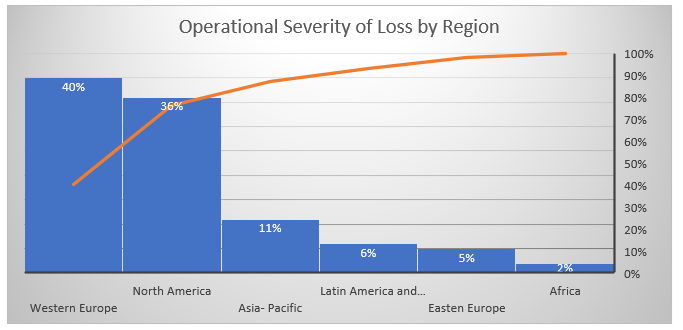
\includegraphics[width=1\linewidth]{ORX report Chat.png}
    \caption{Source: Annual Banking Loss Report ORX global banking database 2024}
    \label{fig:orx-report}
\end{figure}

The analysis in figure \ref{fig:orx-report} shows operational risk losses in the global banking system, revealing that Western Europe 40\% is the most affected region, followed by North America at 36\%. The majority 76\% of losses indicate higher exposure due to regulatory complexity, advanced automated financial systems, and high transaction volumes. Asia Pacific follows with a minimum risk profile of 11\%, as recorded above, and Latin America then accounts for only 6\%. Eastern Europe and Africa record the lowest \% rating, most probably due to underreporting and low banking activities. The cumulative trend shows that high losses are concentrated in developed nations and low-risk profiles in developing nations. 
\newpage
\textbf{Growth of the global banking operational loss database} (2014-2019)
\begin{table}[H]
    \centering
    \begin{tabular}{|c|c|c|c|}
        \hline
        Year & Total number of firms & Cumulative total gross loss (bn) & Cumulative frequency(OR Loss) \\
        \hline
        2014 & 80  & 247.00 & 419,954 \\
        2015 & 85  & 325.00 & 490,044 \\
        2016 & 92  & 371.00 & 566,590 \\
        2017 & 96  & 419.00 & 634,512 \\
        2018 & 97  & 458.00 & 695,139 \\
        2019 & 100 & 482.00 & 778,639 \\
        \hline
    \end{tabular}
    \caption{Summary of Firms, Gross Loss, and Operational Risk Events (2014-2019)}
    \label{tab:summary_table}
\end{table}
The Table \ref{tab:summary_table} was extracted from the ORX 2019 annual report database. From the findings, the participants observed an alarming rate of annual losses attributed to operational risk. As an association, ORX was established by a group of banks to create a global platform for secure and anonymous data exchange. This platform was established to help organisation evaluate their risk profiles and suggest the best possible ways to mitigate and reduce operational risk losses. 

The data in table \ref{tab:summary_table} indicate that cumulative total gross losses rose from \$247 billion in 2014 to \$482 billion in 2019, a nearly 95\% increase over five years. The frequency of operational risk events doubled from approximately 420 thousand events in 2014 to 780 thousand events in 2019. These figures indicate that overall exposure to operational risk is significantly increasing. Banks are facing double losses and higher risk events during this period. The number of firms participating increased from 80 to 100, accounting for a 25\% total increase. This suggests that a wider range of institutions is facing operational risk, contributing to the overall rise in global losses. The increase in both loss amounts recorded and frequency of events indicates that, without effective risk controls, the likelihood of getting high-severity losses will continue to rise.

\textbf{Basel Event Types: ORX Reference Taxonomy}
\begin{figure}[H]
    \centering
    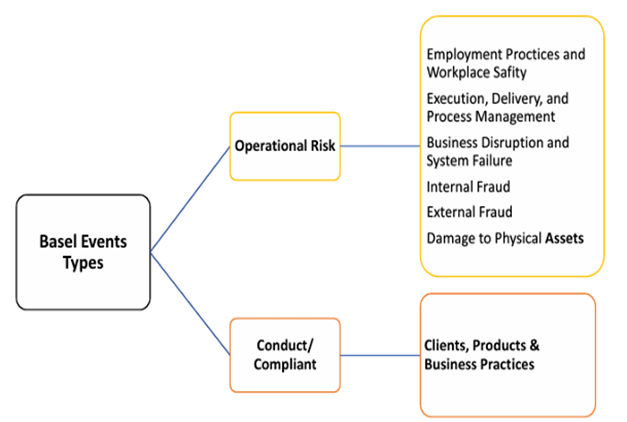
\includegraphics[width=1\linewidth]{Basel Event Types.png}
    \caption{Basel Event Types}
    \label{fig: Basel Event Types}
\end{figure}\\

The figure \ref{fig: Basel Event Types} illustrates the results of Basel Types and an analysis of the ORX Reference Taxonomy level 1s. This presents an essential framework for categorizing operational risk events in the banking and Insurance sector. The event types shown above were introduced under the Basel II framework and classify key risk events into seven broad categories: Internal Fraud, External Fraud, Employment Practices, Clients \& Products, Physical Assets, System Failures, and Process Management. Grouping and categorizing risk events help financial institutions to analyze loss events and implement effective policies to manage operational risk losses. ORX report refines these categories to reflect the evolving risk landscapes, such as cyber risk, third-party risk, and data management. They also break down the conduct and compliance risks into more specific components like financial crime and regulatory compliance. The comparison highlights how ORX's taxonomy simplifies the nature of operational risks, helping firms manage operational risk more effectively in today’s rapidly changing environment.

The rapid expansion of mobile money transfer platforms, digital banking, and Internet banking has led to a rise in operational risk, particularly in developing nations with poor security protocols and outdated banking systems in most companies. Several firms in Zimbabwe are affected by cyberattacks and data breaches every year. Econet Wireless was reportedly hit by a ‘Data Breach’, the suspect threatens to sell Econet's Customer database with 852,791 details of the customers, said the source, ZimDaily News (2025). Another similar incident occurred in 2024 when ZB Financial Holdings, one of Zimbabwe’s largest financial institutions, suffered a ransomware attack in July, resulting in a significant data leak.

Despite repeated attempts to contact ZB for comments, the company has not provided an official response, said the source, TechZim. National Foods lost over \$6 million to cybercriminals who hacked its systems and used phishing emails to deceive the finance manager into transferring funds. The scam involved two foreign suspects posing as a South African financial institution. According to Herald Zimbabwe (2017), Ok Zimbabwe lost 70,000 USD after one of its employees hacked into OK’s Money Wave system and made a transfer into his account. State-owned telecom company Netone claims it lost more than USD 1 million in potential revenue due to alleged fraud by one of its dealers, accused of illegally activating mobile lines without authorization in 2022, said the source, Kukurigo 2025.  According to Statista's report, the global cost of cybercrime is expected to surge in the next four years, rising from \$9.22 trillion in 2024 to \$13.82 trillion by 2028.

This research is essential due to the growing, alarming threat of operational risk in banks, insurance industries, and non-financial institutions. The integration of digital banking, mobile money transactions, and internet-based financial services paved the way for operational risk to those institutions with weak security protocols \parencite{cybersecurity2024}. As we can see from recent cyberattacks, data breaches, and fraud cases affecting major institutions in Zimbabwe, it is clear that many organizations are highly vulnerable. \textcite{madzudzo2021cybersecurity} asserts that global cybercrime costs are expected to increase significantly. 

Understanding the nature of risk is crucial for maintaining financial stability, ensuring regulatory compliance, and fostering consumer trust. To effectively manage these financial threats, organizations must quantify key risk indicators, enabling them to measure and mitigate potential financial losses that could disrupt business operations. A case study conducted by \textcite{ey2025operationalrisk} suggested that by establishing a robust framework to quantify operational risk, organizations across various industries will be better equipped to allocate resources effectively and implement targeted risk mitigation strategies, ultimately reducing potential losses. 

Operational risk is one of the most difficult risks to model. The challenges faced may include quantifying and validating Bayesian network models of operational risk for internal or external reviewers \parencite{zhang2023bayesian}. This research sets out a framework that I believe some other risk professionals may consider when quantifying and validating such models, concerning quantification of the network, probability eliciting, Protocols and bias, Validations of estimates, Structural model building, Risk process mapping and node identification, network structure, conditional probabilities and nodes discretion tables and Model structure validation. Bayesian networks are built upon a causal factor framework, pulling together the known (factors) and unknown (probabilities) into a visual node map to describe each risk process \parencite{ifoa2023operationalrisk}. The factors will be a mixture of firm-specific and external risk drivers.

It has been suggested that under the Basel II Accord, commercial banks have been required to calculate the operational risk capital charges, \parencite{shevchenko2013loss}. The Loss Distribution Approach is one of the suggested standard approaches used to quantify and validate the operational risk and capital charge. The fundamental issue in studying operational risk is the lack of a universal understanding of the actual meaning of operational risk among scholars, theorists, practitioners, and researchers. For this study, we use the definition proposed by the RBZ, and the one adopted in the Accord is “the risk of direct or indirect loss resulting from inadequate or failed internal processes, people, and systems or from external events, and this definition includes legal risk”.  It should be noted that according to this accord, this definition was developed for all financial institutions, Banks, and insurance companies concerning specific risk elements. According to the revised Basel Committee report, “legal risk includes but is not limited to exposure to fines, penalties, or punitive damages resulting from supervisory actions, as well as private settlements. 

How to construct a Bayesian Network diagram that establishes a relationship between the necessary operational risk attributes is not yet fully resolved. According to \textcite{basel2021principles}, and \textcite{difrancesco2023bayesian}, financial institutions must develop, implement, and maintain an operational risk management framework fully integrated into the institution’s overall risk management processes. Therefore, we need to clarify to what extent the quantifying methodologies allow the construction and validation of a model that considers the main features of all operational risks. The Basel Committee on Banking Supervision reviewed the operational risk management framework adopted by an individual institution and stated that a bank will depend on a variety of factors, including the nature, size, complexity, and risk profile of the bank. The losses generated by the operational risk are identified and connected under the international standards for the seven-event types, internal fraud, external fraud, employment practices and the safety of the working place, the clients, the products, and the commercial practices; the tangible assets loss, the activity rupture and the inadequate systems functioning and the process execution, the delivery, and management. 

This study aims to find better ways to understand and manage key risk indicators that are being faced in the financial sector industry. Using the Bayesian Network modeling, to create a visual map showing how different operational risk factors are connected and how they influence each other. This study also aims to figure out which factors are the most important in causing problems and how changes in one factor might affect other factors. This makes it easier for organizations to predict potential risks and take action to reduce them before they become bigger issues. Essentially, it's about building a smart Bayesian system that helps identify, measure, and validate the key causes of risks, leading to more effective and proactive risk management. Bayesian Networks can be effectively machine-learned from an operational risk incident database, enabling a risk manager to measure and report operational risk effectively and giving them the ability to manage and make informed decisions.

Several Authors have extensively explored the process and loss event analysis using the Bayesian Network modeling approach to better analyze and understand operational risk related to specific processes or sub-risk areas. Therefore, further research is needed to elaborate on how the Bayesian Network models can be constructed and learned, and then be applied in the effective management of operational risk at a bank or at an insurance company. How can these models be used in risk management and not just for regulatory reporting or risk calculation purposes? Also, how the models can allow for risk management to be viewed at a bank-wide or bank-unit-wide level and not just specific to a process or sub-risk type.

\section{Statement of the problem}

Operational risk is significant in all financial institutions, and it’s a major critical concern for financial institutions, as it can lead to substantial losses resulting from failures in internal processes or external events. Operational risk is hard to quantify, given the presence of heavy-tailed loss distribution \parencite{johanna2022capital}, and the lack of data usually for low-frequency and high-impact losses  \parencite{article}.  Despite regulatory advancements, such as the Basel II and Basel III Accords, operational risk modeling remains challenging due to the complexities in identifying, quantifying, and validating the interconnected causal relationships between risk factors. While traditional methods like the Loss Distribution Approach (LDA) are widely used, they do not fully quantify the key operational risk factors. 

Amongst the more sophisticated methods developed are linear models such as time series, econometric, and empirical actuarial models. These models rely on historical data to predict future values based on past trends. According to \textcite{dutta2006tale}, operational Risk losses often exhibit fat-tailed distributions, which means extreme losses would occur more frequently than would be predicted by linear models. Therefore, the relationship between variables in operational risks is non-linear and complex, making it difficult to model accurately using linear models. However, despite extensive research on operational risk, evidence for quantifying and validating key operational risk factors remains unclear.

Bayesian Network (BN) modeling presents a promising framework for addressing this gap by providing a probabilistic, causal structure that links risk factors in a visual node map. BNs allow for overcoming these hurdles as they combine qualitative data from experts and relevant quantitative data. Even with advances in modeling, challenges remain when it comes to building and validating these risk frameworks. It’s not always easy to define how different risk factors are connected, estimate the likelihood of certain events, or ensure that the model works in real-world scenarios. For many financial institutions, integrating these models into daily risk management, not just for ticking regulatory boxes, can be difficult because of how complex and technical they can be.

This study addresses the problem of developing the Bayesian Network framework for operational risk management, mainly focused on quantifying and validating causal relationships among key risk factors. The model seeks to enhance the understanding of how these models can be practically applied, enabling financial institutions to not only meet regulatory requirements but also improve proactive risk management at both the bank-wide and unit-specific levels.

\section{Aims and Objectives}
The primary aim of the study is to develop a framework using Bayesian Network (BN) modeling to identify, quantify, and measure operational risk in several business lines of commercial banking. The objective is to help risk professionals quantify and validate causal relationships between different operational risk factors. Therefore, by doing so, the study seeks to improve the accuracy and effectiveness of risk measurement and management practices.
\section{Main Objectives}
These objectives aim to establish a comprehensive framework for modeling operational risk using Bayesian Networks, allowing for the quantification, validation, and interpretation of causal relationships between risk factors.
 \subsection{Primary Objectives}
These objectives aim to establish a comprehensive framework for modeling operational risk using Bayesian Networks, allowing for quantifying, validating, and interpreting causal relationships between risk factors.
\begin{enumerate}
    \item Construct a Bayesian Network (BN) Framework: To develop a BN diagram that accurately establishes relationships between the key operational risk attributes, illustrating how different factors influence each other.
    \item Quantify the Network and Validate Estimates; To quantify the network by estimating probabilities associated with different risk scenarios and events
    \item Validate the Model Structure; To validate the Bayesian Network model structure, ensuring that it accurately represents the causal relationships and can be used for effective risk management.
\end{enumerate}

\subsection{Research questions}
To manage operational risk effectively, the factors thought to influence the key risk factors should be identified and addressed. Ideally, the research questions are designed to explore major aspects of using Bayesian Networks for operational risk modeling, from constructing the framework to validating its structure and probability estimates. 

\begin{enumerate}
    \item How can the Bayesian Network (BN) diagram, which represents the relationships between key operational risk attributes, be constructed effectively?
    \item What are the critical steps to quantify the dependency between risks, and which methods can be used to quantify the network and accurately estimate the probabilities associated with various operational risk factors?
    \item What are the critical steps for mapping the risk process and identifying key nodes within the Bayesian Network structure for operational risk modeling?
    \item What role do conditional probability tables and nodes' discretion play in defining the relationships within a Bayesian Network for operational risk?
    \item What are the challenges in using Bayesian Networks for operational risk modeling, and how can they be addressed through model validation and structural refinement?
\end{enumerate}

\section{Justification/Rationale or Significance of Research}
The research will be of significance to different stakeholders as follows: 

\subsection{To Banks and other organizations: }
Banks will be able to measure and quantify the key operational risk and approximately estimate the capital charge that might be required in case of severe risk occurring, and also to measure the level of risk awareness within the organization.  To other organizations, the research will represent a proxy of guidance for their operational risk management programs. The study is significant to both stakeholders and education 5.0, as the following shows the importance of choosing the Bayesian Method as a tool used to assess the impact of operational risk.

According to Yew (2020), the graphical presentation of BNs aids the understanding of the causal structure. It presents the risk profile of the company intuitively, improving management's knowledge of, and hence participation in, the management of operational risk.  This study provides a robust framework for modeling and managing operational risks, allowing organizations to better understand and mitigate risks, leading to more informed decision-making.

Traditional linear models may struggle to capture the complex, non-linear dependencies often found in operational risk scenarios. Conditional probabilities can be quantified to take into account the impact of controls and mitigating actions, thus providing a platform for what-if analysis, helping to analyze the effect of specific controls and identifying which controls have the most impact on resultant loss, which can be used in future planning and investment choices Therefore, using the Bayesian Networks helps overcome these limitations, providing a more flexible and sophisticated approach to modeling risk factors and their interactions.

Operational risk losses often have "fat-tailed" distributions, meaning that extreme losses occur more frequently than expected under standard models. The proposed Bayesian Network framework can better accommodate and model these extreme events, offering a more realistic assessment of risk.

Financial institutions face regulatory requirements for quantifying and managing operational risk. This study's framework can help firms meet regulatory standards by providing a validated model for risk quantification, which is essential for calculating capital reserves and demonstrating compliance with industry guidelines \parencite{IMF2023_Zimbabwe}.

Bayesian decision networks provide a cost-benefit analysis of risk controls, where the optimal controls are determined within a scenario analysis framework. The Bayesian Network approach allows for stress testing and scenario analysis, enabling organizations to test how the models perform under different conditions.  Scenario building is identifying the critical factors that contribute to an adverse event and crafting a narrative that briefly describes the circumstances and consequences if it were to happen. This will help to identify whether the Bayesian Network can effectively capture the impact of catastrophic events or emerging risks.
\subsection{To the Researcher}
The researcher will gain valuable insights from a different angle of risk management to augment his valuable banking experience and hopes to expand and broaden his knowledge. The academic world will benefit from the valuable, diverse literature as applied in a real organization
\subsection{Practical Implications for Operational Risk Managers:}
The framework provides operational risk managers with practical tools for mapping risk processes, identifying key risk factors, and validating risk models. One of the key advantages of Bayesian Network models is that they can easily be visualized with the use of the node or factor map \parencite{article}. These visuals are easy to understand for any stakeholder in the business, allowing a broader range of stakeholder challenges. It is widely accepted that this will enhance the understanding of each business process and its associated risks and controls, providing a closer link between risk measurement and risk management approaches.

One of the advantages of using a Bayesian network as a modeling tool is that it can answer queries that are both predictive and diagnostic \parencite{sanford_bayesian_2012}. For example, a predictive query may ask, “What is the probability of a payment failure given that a loan is being processed?”, whilst a diagnostic query may ask, “What is the most probable transaction type processed given that a payment failure occurred?”. Experts agree that, having observed the state of an effect node, such as a payment failure, inference can be carried out to show the probable states of the causal nodes within the network modeling in structured finance operations. 

The Bayesian Network provides an effective technique for quantifying and modeling operational risk \parencite{zhao_data_2024}. The model can be utilized across several areas of study, including areas such as improving operational continuity, evaluating response strategies, and assessing newer risks like those related to cybersecurity and climate change. In addition, the Bayesian Framework allows better strategic decisions, as it enables the assessment of various management responses under different operational risk conditions.
 
\subsection{Assumptions for Learning the Causal Structure}
The Causal Sufficiency Assumption and the Markov Assumption are foundational theories for applying Bayesian Networks (BNs) practically. According to \textcite{Chobtham2020}, and \textcite{Wu2023}, the Causal Sufficiency Assumption states that no unobserved variables act as common causes of two or more observed variables within the domain. This assumption is critical for ensuring that observed dependencies and independencies in the data accurately reflect the true causal structure rather than omitted confounders.

The Markov Assumption, integral to the BN framework, asserts that a variable is conditionally independent of its non-descendants given its parents and this property enables the factorization of the joint probability distribution into conditional probabilities, facilitating efficient computation and inference. When the Causal Sufficiency Assumption is violated, the Markov property may fail, as unobserved variables introduce dependencies not accounted for in the model. Such violations can be seen as unexpected conditional dependencies in the data, undermining the reliability of the BN’s conclusions about causal or probabilistic relationships.

To address the challenges posed by latent variables, methodological advancements have focused on techniques such as instrumental variables (IVs), which exploit exogenous variation to estimate causal effects in the presence of unobserved confounding. Ongoing research extends these principles to develop tests for detecting latent variables in constrained settings and to enhance BN frameworks through hybrid models, such as structural equation models (SEMs), which explicitly incorporate latent variables. These approaches aim to reconcile the theoretical precision of BNs with the complexities of real-world data, where unobserved variables are pervasive.

The Causal Sufficiency and Markov Assumptions provide a powerful framework for modeling probabilistic and causal relationships; their real-world applicability is assumed to be effective in real-world data as according to  \textcite{Fazio2024}, \textcite{Asgari2024}, and \textcite{Miklin2021}. Acknowledging these limitations underscores the importance of integrating complementary methods—such as IVs, latent variable modeling, or hybrid SEMs—to enhance the robustness of BN-based analyses.

\subsection{Scope of Research/Delimitation of the Study}
Operational risk has become the major trending topic in financial institutions, but from all the findings available, there is no significant research that has been done to quantify and characterize operational risk. There are limited studies on operational risk management, and most studies have tended to focus on traditional methods to model operational risk in financial services organizations. 

Developing a Bayesian modeling framework is the underlying theme of this study, and this study will provide a robust framework for managing operational risks, allowing organizations to better understand and mitigate risks, leading to more informed decision-making. Research suggests that BN framework can be structured in such a way to have the various operational risk factors cascade into an overall loss, thus allowing risk capital to be specified. The built-in causal relationships within Bayesian Networks make them effective tools for detecting and assessing the consequences of operational loss incidents. This aligns with the key criteria expected of operational risk models in the financial sector.

\section{Definition of Key Terms}
\subsection{Bayesian Network}
Bayesian networks are directed acyclic graphs that allow efficient and effective representation of the joint probability distribution over a set of random variables \parencite{sanford_operational_2015}. In this graphical structure, nodes correspond to random variables, while edges illustrate direct relationships between them. The network captures conditional independencies by ensuring that each variable is independent of its non-descendant variables, provided the values of its parent nodes are known. \textcite{unknown} and Atakan (2019) defined the Bayesian Network as a Probabilistic Graphical Model (PGM) that represents conditional dependencies between random variables through a Direct Acyclic Graph (DAC), which can be applied in many fields, particularly for operational risk in financial institutions. 
\subsection{Operational Risk}
Operational risk (OR) is defined by the Basel Committee on Banking Supervision (BCBS) as the risk of loss resulting from “inadequate or failed internal processes, people and systems or from external events”. It is a fundamental element of risk management at banks \parencite{bcbs2004basel2}. The actual definition of operational risk presented by the Basel II becomes the international standard definition recognized. This ascertains that Operation risk can be classified as the uncertainties and potential hazards a company faces while conducting its day-to-day business operations. Unlike systematic risk, which stems from external forces such as economic or political events, operational risk is primarily linked to an organization's internal operations, decision-making processes and internal system failures.
\subsection{Quantification of operational risk }
Quantification of operational risk can be described as the process of measuring losses and assessing the potential losses from the identified key risk indicators, Internal Failures, Human errors, System Failures, Disasters, and external business disruptions \parencite{kim2021system}. This process involves the use of probability elicitation and probability graphical models to represent and analyze the dependencies between various risk factors and events. This method uses combined historical data, expert judgment for probability elicitation, and scenario analysis to update risk probabilities as new data becomes available. This effectively ensures more accurate risk assessment and mitigation strategies.
\subsection{Scenario Analysis}
According to \textcite{fenton2010managing}, Bayesian decision networks provide a cost-benefit analysis of risk controls, where the optimal controls are determined within a scenario analysis framework. The Bayesian Network approach allows for stress testing and scenario analysis, enabling organizations to test how the models perform under different conditions \parencite{rippel_operational_2011}. Scenario development involves pinpointing key elements that could lead to a negative event and constructing a concise description outlining the context and potential outcomes should the event occur. This will help to identify whether the Bayesian Network can effectively capture the impact of catastrophic events or emerging risks.
\subsection{Casual Analysis}
Scholars have suggested that causal analysis is an effective way to understand what causes operational losses in the business environment. Causal analysis, just like scenario analysis, looks at the historical losses and updates the likelihood of different risk factors being responsible \parencite{andersen2016causal}. Causal analysis analyzes in a better way, rather than predicting losses, diving much deeper into the causes and interrelationships between variables. Taking this into consideration, if a Bank is facing losses and wants to prevent further losses, it needs to identify the main causes of the major losses.  Through a deep analysis, the bank can easily find out which risk factors are causing the losses, Maybe, data quality, weak security protocols, and system failure have the biggest impact. This plays a crucial role in helping companies improve their systems and reduce risks more effectively. 
\subsection{Loss Distribution Approach}
The Loss Distribution Approach is a statistical technique that estimates the distribution of losses based on historical data \parencite{wang_method_2017}. \textcite{hadley_selection_2019} argues that LDA assumes that operational losses are driven by two independent factors, which are as follows: the frequency and the severity of the event. The frequency is the number of loss events that occur in a given period, such as a year. The LDA works like this: we list out all the things that could go wrong for a company, such as Fraud, system glitches, execution errors, and legal issues. Then, we figure out how likely each event is and how much money it will cost. then create a sort of overall Bayesian map showing the possible losses and decide how much money it needs to have on hand (Kind of like a safety net) to cover unexpected financial loss from the potential issues.
\newpage
\textbf{Overview of the this research analysis}
\begin{itemize}
    \item \textbf{Chapter 1 - Introduction} - This chapter provides an overview of the study, covering the aims, objectives, statement of the problem, significance of the study, delimitation, and limitations.
    
    \item \textbf{Chapter 2 - Literature Review} - This section examines the literature relevant to related studies and theoretical background.
    
    \item \textbf{Chapter 3 - Methodology} - This chapter describes the research methodology, including analytical tools and procedures used to conduct the study.
    
    \item \textbf{Chapter 4 - Data Analysis \& Results} - This section presents the analysis of data and interpretation of the results.
    
    \item \textbf{Chapter 5 - Conclusion, Discussion, Recommendations, and Limitations} - The final chapter covers the summary, conclusions, and recommendations derived from the data analysis and interpretation of results.
\end{itemize}
\newpage
\section{Chapter Summary}
This chapter serves as an introduction to this project on operational risk modeling within financial institutions, emphasizing the challenges associated with accurately identifying, quantifying, and validating key risk factors. The chapter discussed the Background of the Study, highlighting the impact of operational risk losses, limitations of traditional modeling methods, and the potential of Bayesian Network (BN) modeling to address these challenges by mapping complex causal relationships among risk factors. 

The Problem Statement addresses the need for a robust framework that goes beyond regulatory compliance, aiming to support proactive risk management through the integration of BN models. The Objectives and Aim of the Study outline the goals of developing and validating a Bayesian framework for quantifying and understanding operational risk factors and enhancing its practical application for financial institutions. The Delimitation of the Study defines the scope, focusing on key operational risk factors within the context of a Bayesian Network structure. Lastly, the Layout of the research provides an overview of the research structure.

The next chapter to follow is going to discuss the relevant literature and theoretical frameworks related to operational risk and Bayesian Network modeling.

